\documentclass{beamer}

\mode<presentation>{
\usetheme{Madrid}
%\usecolortheme{beaver}
}
\usepackage[utf8]{inputenc}
\usepackage{default}
\usepackage[portuguese]{babel}
\usepackage{pgfplots}
\pgfplotsset{/pgf/number format/use comma,compat=newest}
\usepackage{color}
\usepackage{amsmath,amsfonts,amssymb}
\usepackage{hyperref}
\usepackage{tikz}

%\usebackgroundtemplate{%
%\tikz\node[opacity=0.05] {
\includegraphics[height=\paperheight,width=\paperwidth]{logoh_2.png}};}


\title[Improving Load, Performance and Stress Evolutionary Testing using a Hybrid Metaheuristic Approach]{Improving Load, Performance and Stress Evolutionary Testing using a Hybrid Metaheuristic Approach}
\author[Gois, F. N.]{Fraancisco Nauber Bernardo Gois}
\institute[Unifor]{Universidade de Fortaleza}
\date{\today}

\begin{document}

\begin{frame}
 \maketitle
\end{frame}

\begin{frame}
\frametitle{Sumário}
 \tableofcontents
\end{frame}


\section{Advisors}
\begin{frame}
\frametitle{Advisors}
\large{
\begin{itemize}
\item Advisor: Pedro Porfírio Muniz de Farias
\item Co-Advisor: André Luís Vasconcelos Coelho
\end{itemize}
}
\end{frame}




\section{Introduction}
\begin{frame}
\frametitle{Introduction}
The purpose of this research is to propose and investigate the pros and cons of a novel hybrid metaheuristc approach using  Genetic Algorithms, Simulated Annealing and Tabu Search to automatically perform load, performance and stress testing.
\end{frame}


\begin{frame}
\frametitle{Research Activities}
\begin{figure}[H]
\centering
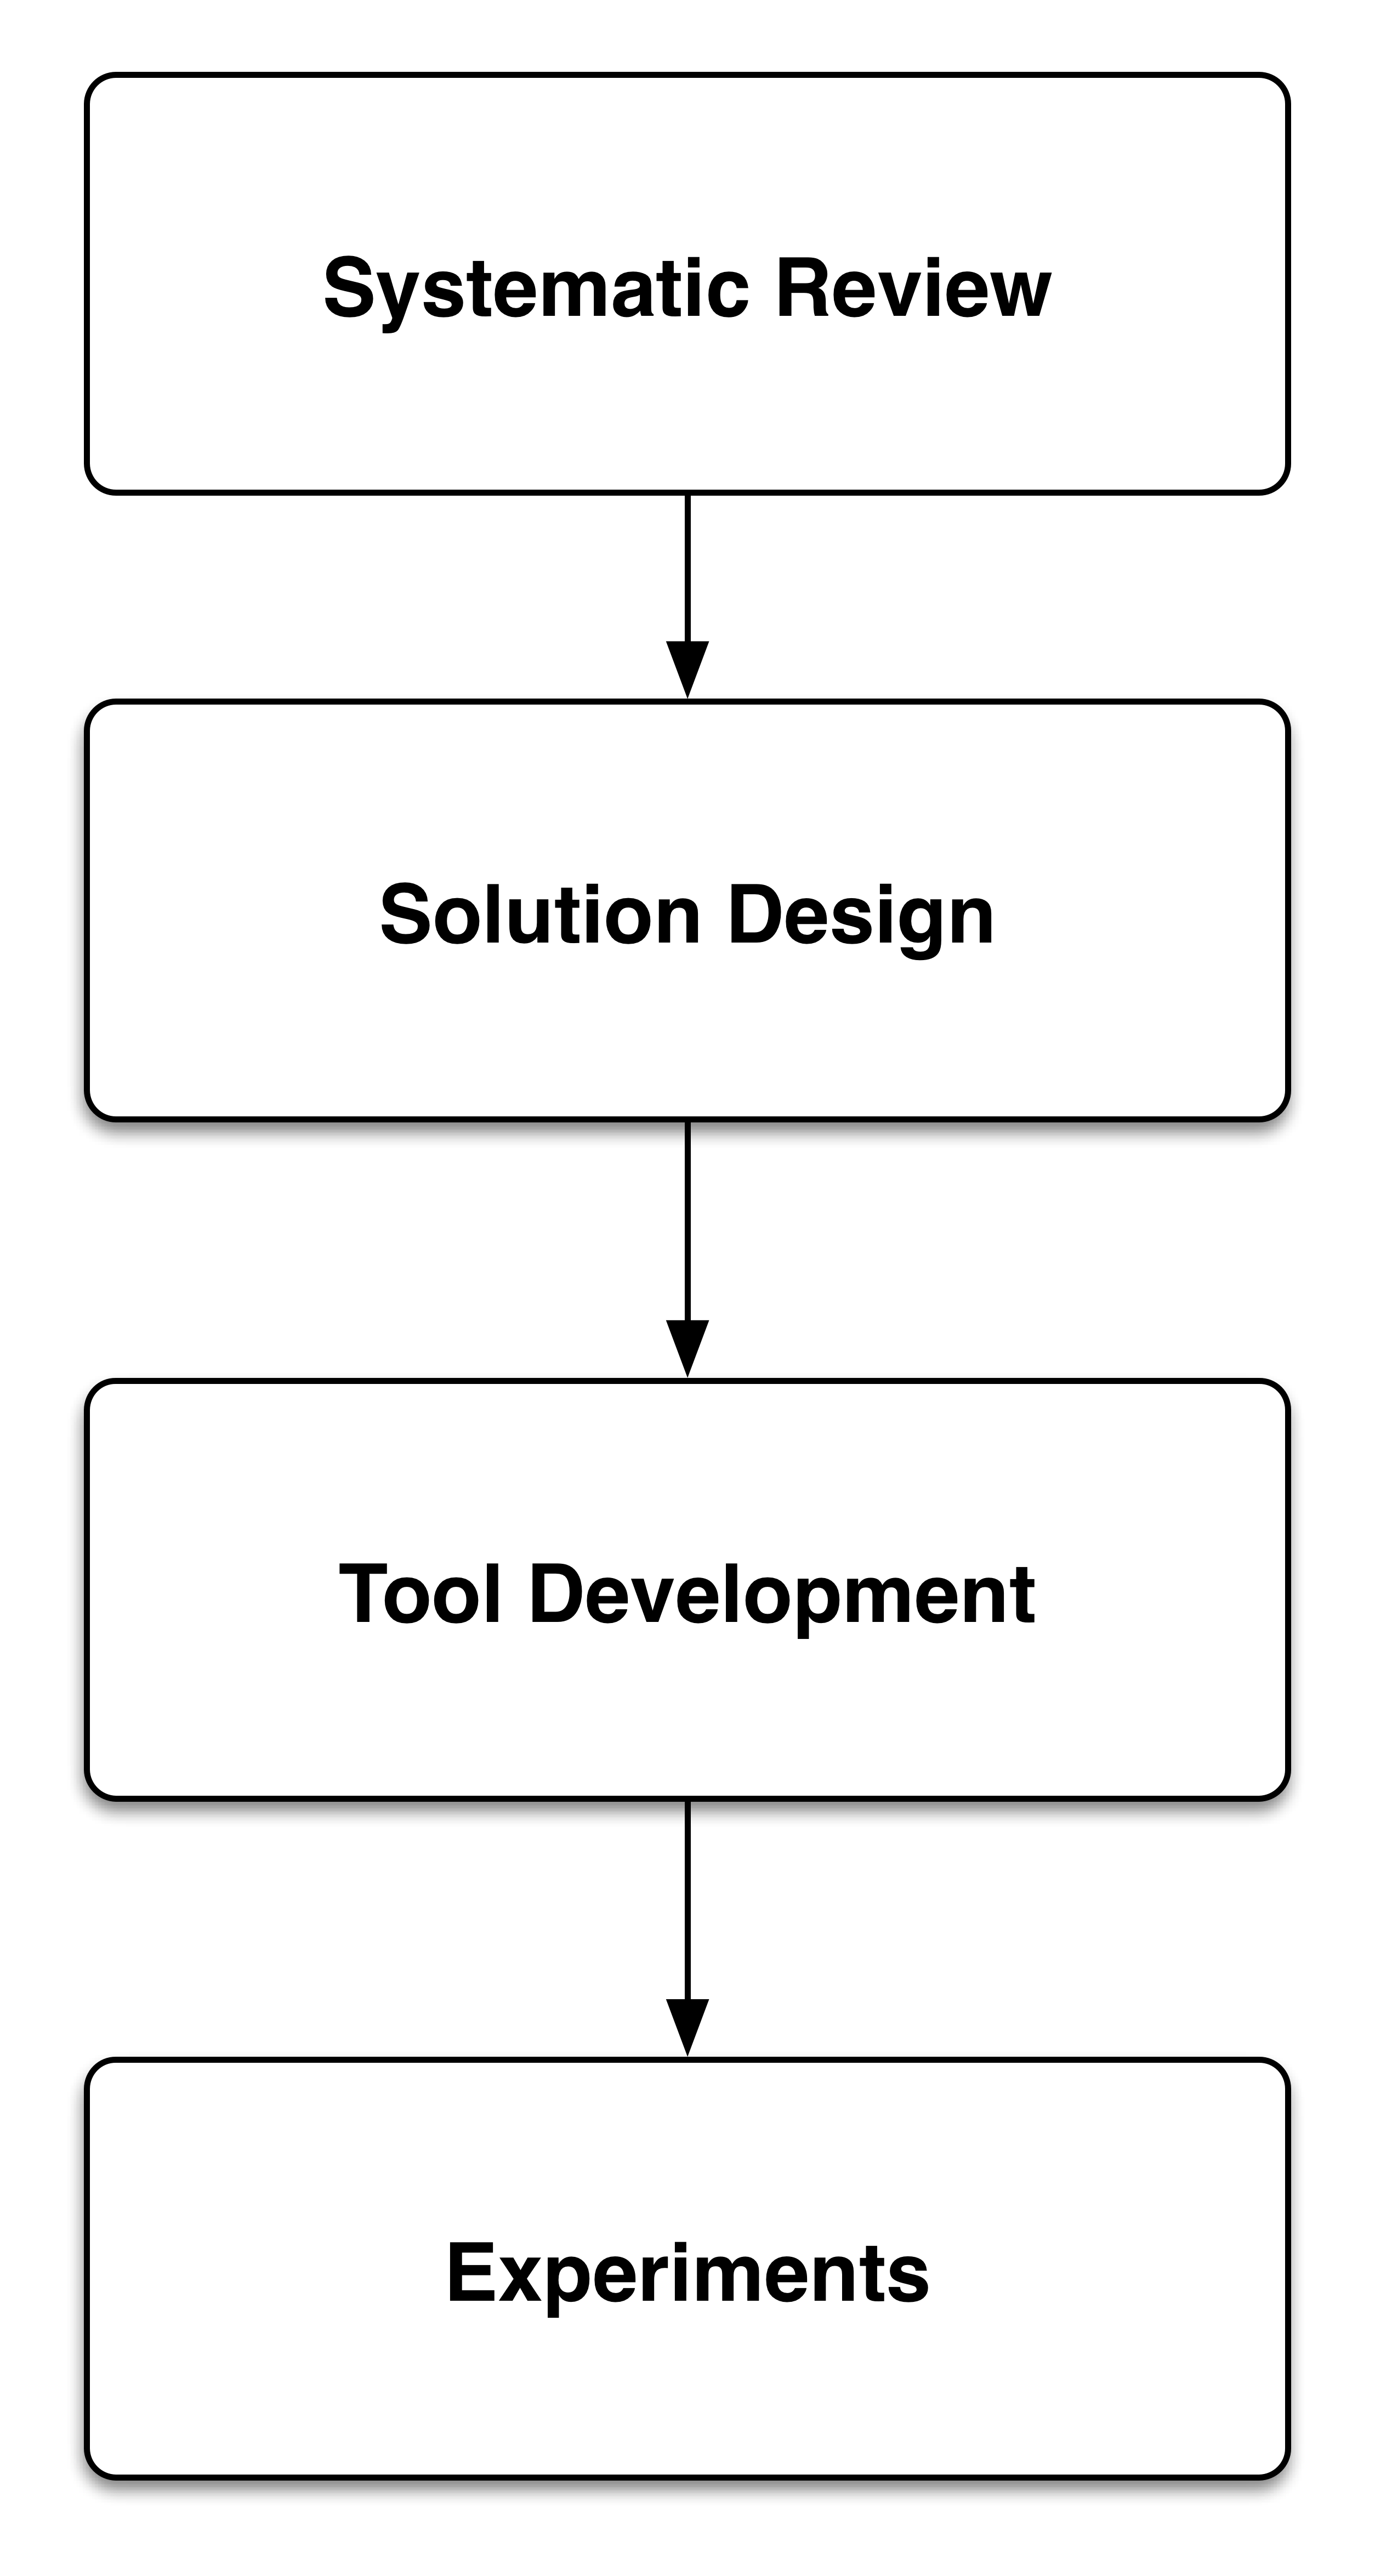
\includegraphics[width=0.3\linewidth]{schedule.PNG}
\end{figure}
\end{frame}

\section{Systematic Review}


\begin{frame}
\frametitle{Bibliography Search Strategy}
\begin{figure}[H]
\centering
\includegraphics[width=0.5\linewidth]{StateofArt.PNG}
\caption{Search Strategy}
\end{figure}
\end{frame}



\begin{frame}
Search terms:
\begin{itemize}
\item Stress Testing: Search-based Testing, Genetic Algorithms, Stress Testing, Test Tools, Test Automation, Empirical Analysis, Denial of Service, Ramp-Up time, Think Timer,  Response Time, Bandwidth Throttle, Dynamic Stress Testing, Evolutionary, Heuristic, Search-Based, Metaheuristic. optimization, genetic algorithms, genetic programming.

\end{itemize}
\end{frame}



\begin{frame}

\begin{itemize}
\item Performance Testing: Performance Testing, Web-based Systems, Software Testing, Model-Based Testing, Software Product Line, Regression Testing, Test Failure Prediction, Genetic Metric Selection.
\item Load Testing: Markov chain,  Automatic Test Case Generation Algorithms, Domain-based reliability measure, Fault detection, Load Test suites, load testing, Reliability, Resource allocation mechanisms, Software testing, System degradation.
\end{itemize}
\end{frame}

\section{Load, Performance and Stress Tests}

\begin{frame}
\frametitle{Load, Performance and Stress Tests}
\begin{figure}[H]
\centering
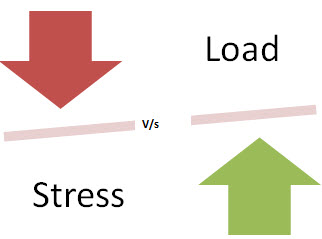
\includegraphics[width=0.7\linewidth]{StressTesting1.jpg}
\end{figure}
\end{frame}


\begin{frame}
\frametitle{Load, Performance and Stress Tests}
The Performance Test aims at verifying a specified system performance. This kind of test is executed by simulating the access of hundreds or more simultaneous users over a defined time interval. The purpose of this test is to demonstrate that the system meets its performance objectives \cite{DiLucca2006}\cite{Sandler2004}.
\end{frame}

\begin{frame}
\frametitle{Load, Performance and Stress Tests}
In load tests, the system is evaluated in pre-defined load levels. The aim of this test is to reach the performance targets for availability, concurrency, throughput and response time of the system. Load Test is the closest to real application use \cite{Molyneaux2009}.
\end{frame}


\begin{frame}
\frametitle{Load, Performance and Stress Tests}
Stress test verifies the system behaviour against heavy workloads, being executed to evaluate a system beyond its limits, validate system response in activity peaks and verify whether the system is capable of recovering from these conditions \cite{Sandler2004}.
\end{frame}

\begin{frame}
\frametitle{Load, Performance and Stress Tests-90 Percentile Line}
\begin{figure}[H]
\centering
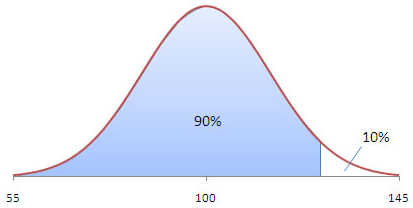
\includegraphics[width=1\linewidth]{90percentile.png}
\end{figure}
\end{frame}

\section{Types of Workloads}

\begin{frame}
\frametitle{Descriptive WorkLoad}
\begin{figure}[H]
\centering
\includegraphics[width=0.6\linewidth]{workloadmodel1.png}
\end{figure}
\end{frame}


\begin{frame}
\frametitle{Generative WorkLoad}
\begin{figure}[H]
\centering
\includegraphics[width=0.6\linewidth]{workloadmodel2.png}
\end{figure}
\end{frame}


\section{Evolutionary Tests}

\begin{frame}
\frametitle{Evolutionary Tests}

\begin{itemize}
\item The main objective of evolutionary testing in performance,stress and load tests is to find test scenarios which produce execution times violating the timing constraints specified. If a temporal error is found, the test was successful \cite{Sullivan}. 

\item The application of evolutionary algorithms to load, performance and stress tests involves finding the best and worst case execution times (BCET, WCET) to determine if timing con- straints are fulfilled \cite{Afzal2009}.
\end{itemize}

\end{frame}


\section{Hybrid Metaheuristic}

\begin{frame}
\frametitle{Hybrid Metaheuristic}
\begin{figure}[H]
\centering
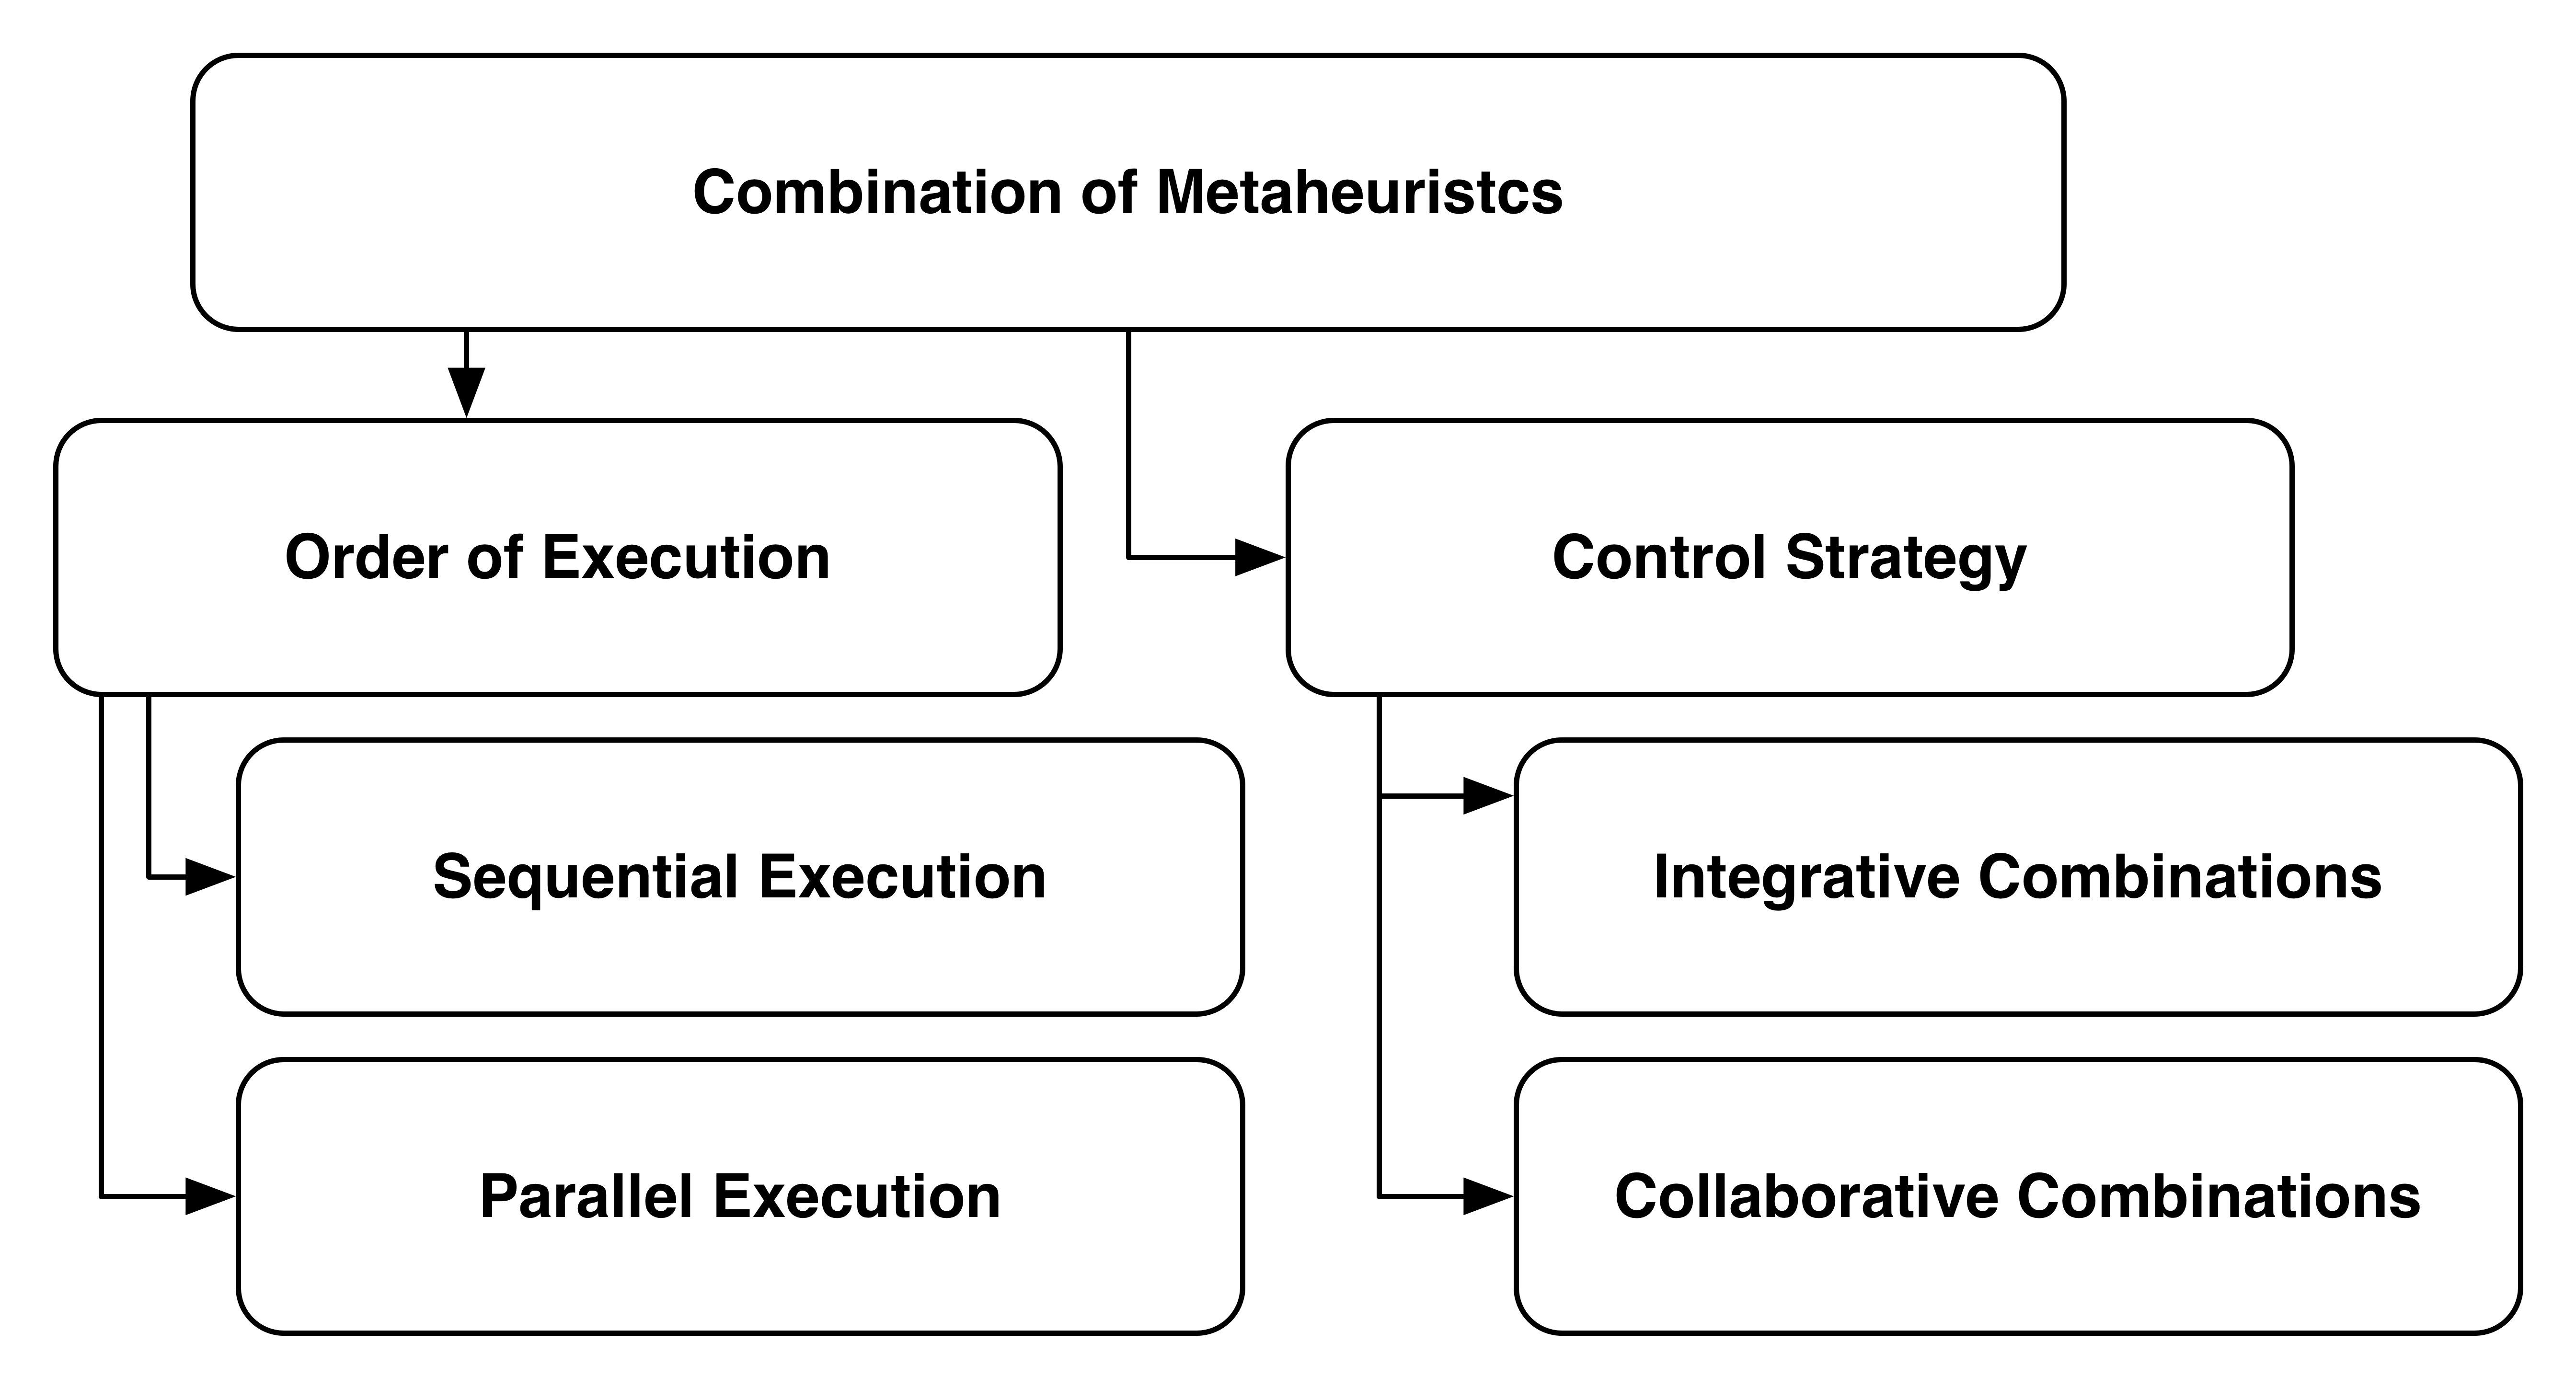
\includegraphics[width=1\linewidth]{metaheuristc2.png}
\caption{Categories of metaheuristc combinations}
\end{figure}
\end{frame}


\section{Search Based Tests}

\begin{frame}
\frametitle{Search Based Tests-Afzal Study}
\begin{figure}[H]
\centering
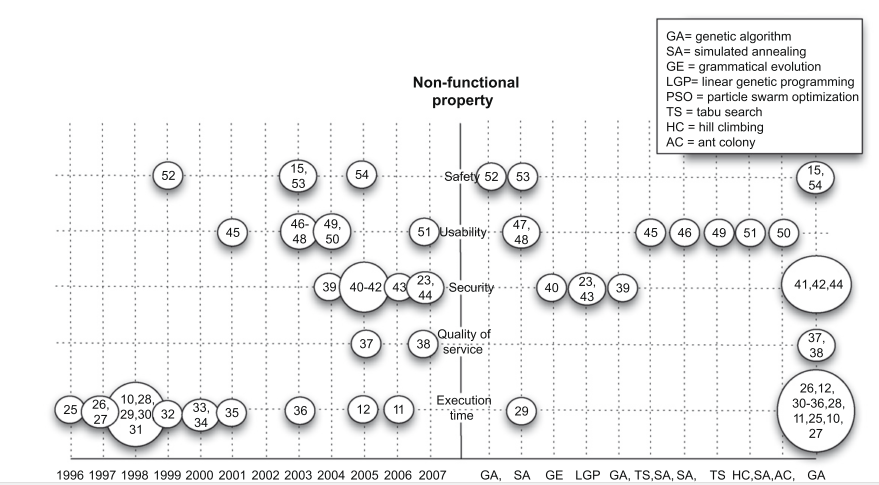
\includegraphics[width=1\linewidth]{afzal.png}
\caption{Distribution of NFSBST research over range of applied metaheuristics and time period  \cite{Afzal2009}}
\end{figure}
\end{frame}





\begin{frame}
\frametitle{Search Based Load, Performance and Stress Tests}
\begin{figure}[H]
\centering
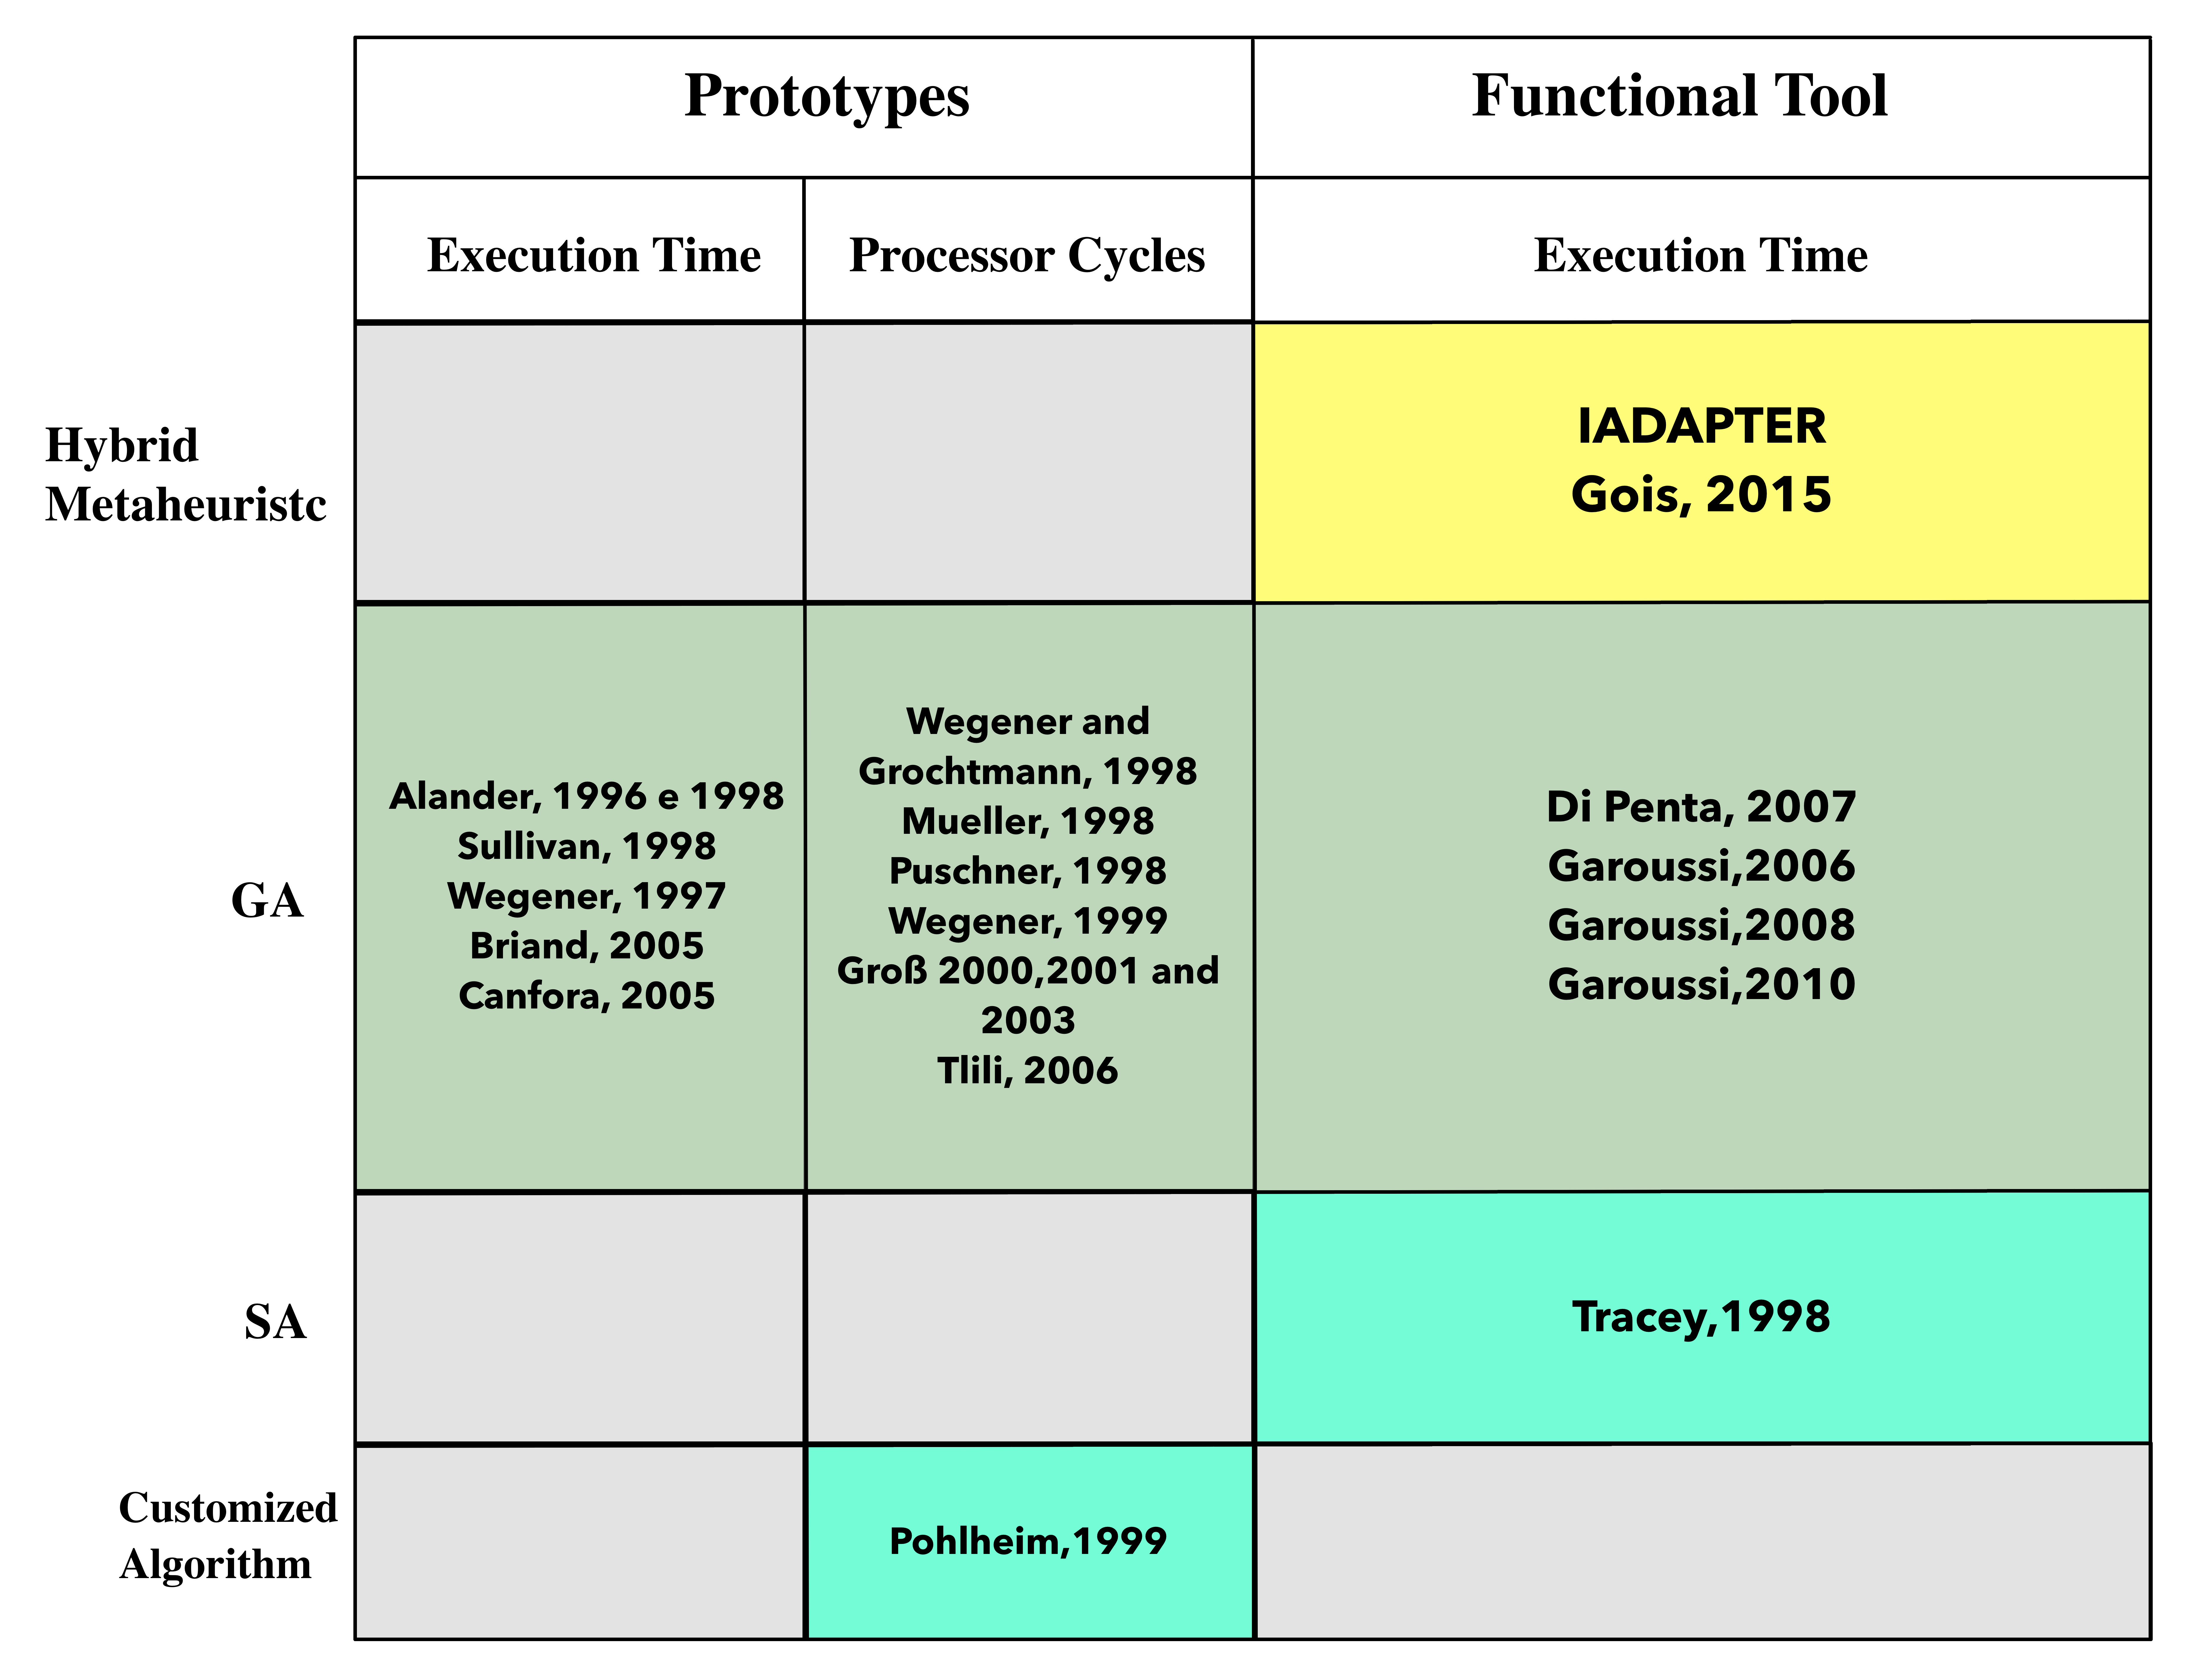
\includegraphics[width=0.8\linewidth]{comparativo1.png}
\end{figure}
\end{frame}


\section{IAdapter}

\begin{frame}
\frametitle{IAdapter}
\begin{figure}[H]
\centering
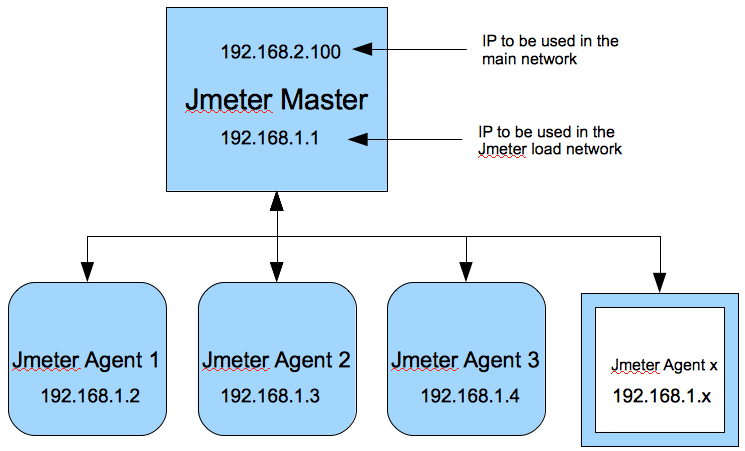
\includegraphics[width=1\linewidth]{jmeter-distributed-structure.png}
\end{figure}
\end{frame}




\begin{frame}
\frametitle{IAdapter}
\begin{figure}[H]
\centering
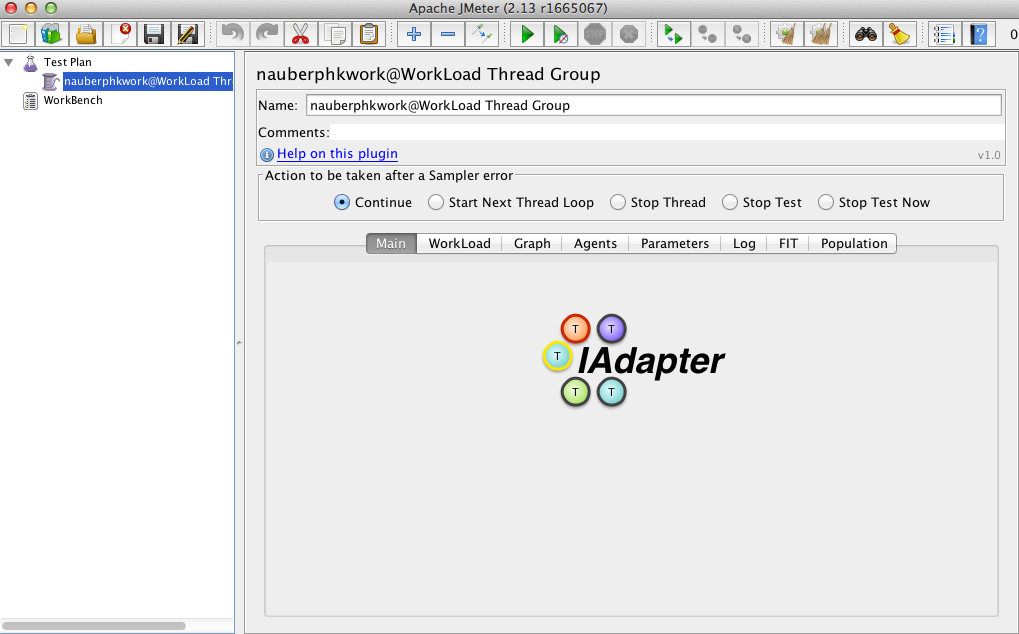
\includegraphics[width=1\linewidth]{iadapter1.png}
\end{figure}
\end{frame}


\begin{frame}
\frametitle{IAdapter-Independent approach}
\begin{figure}[H]
\centering
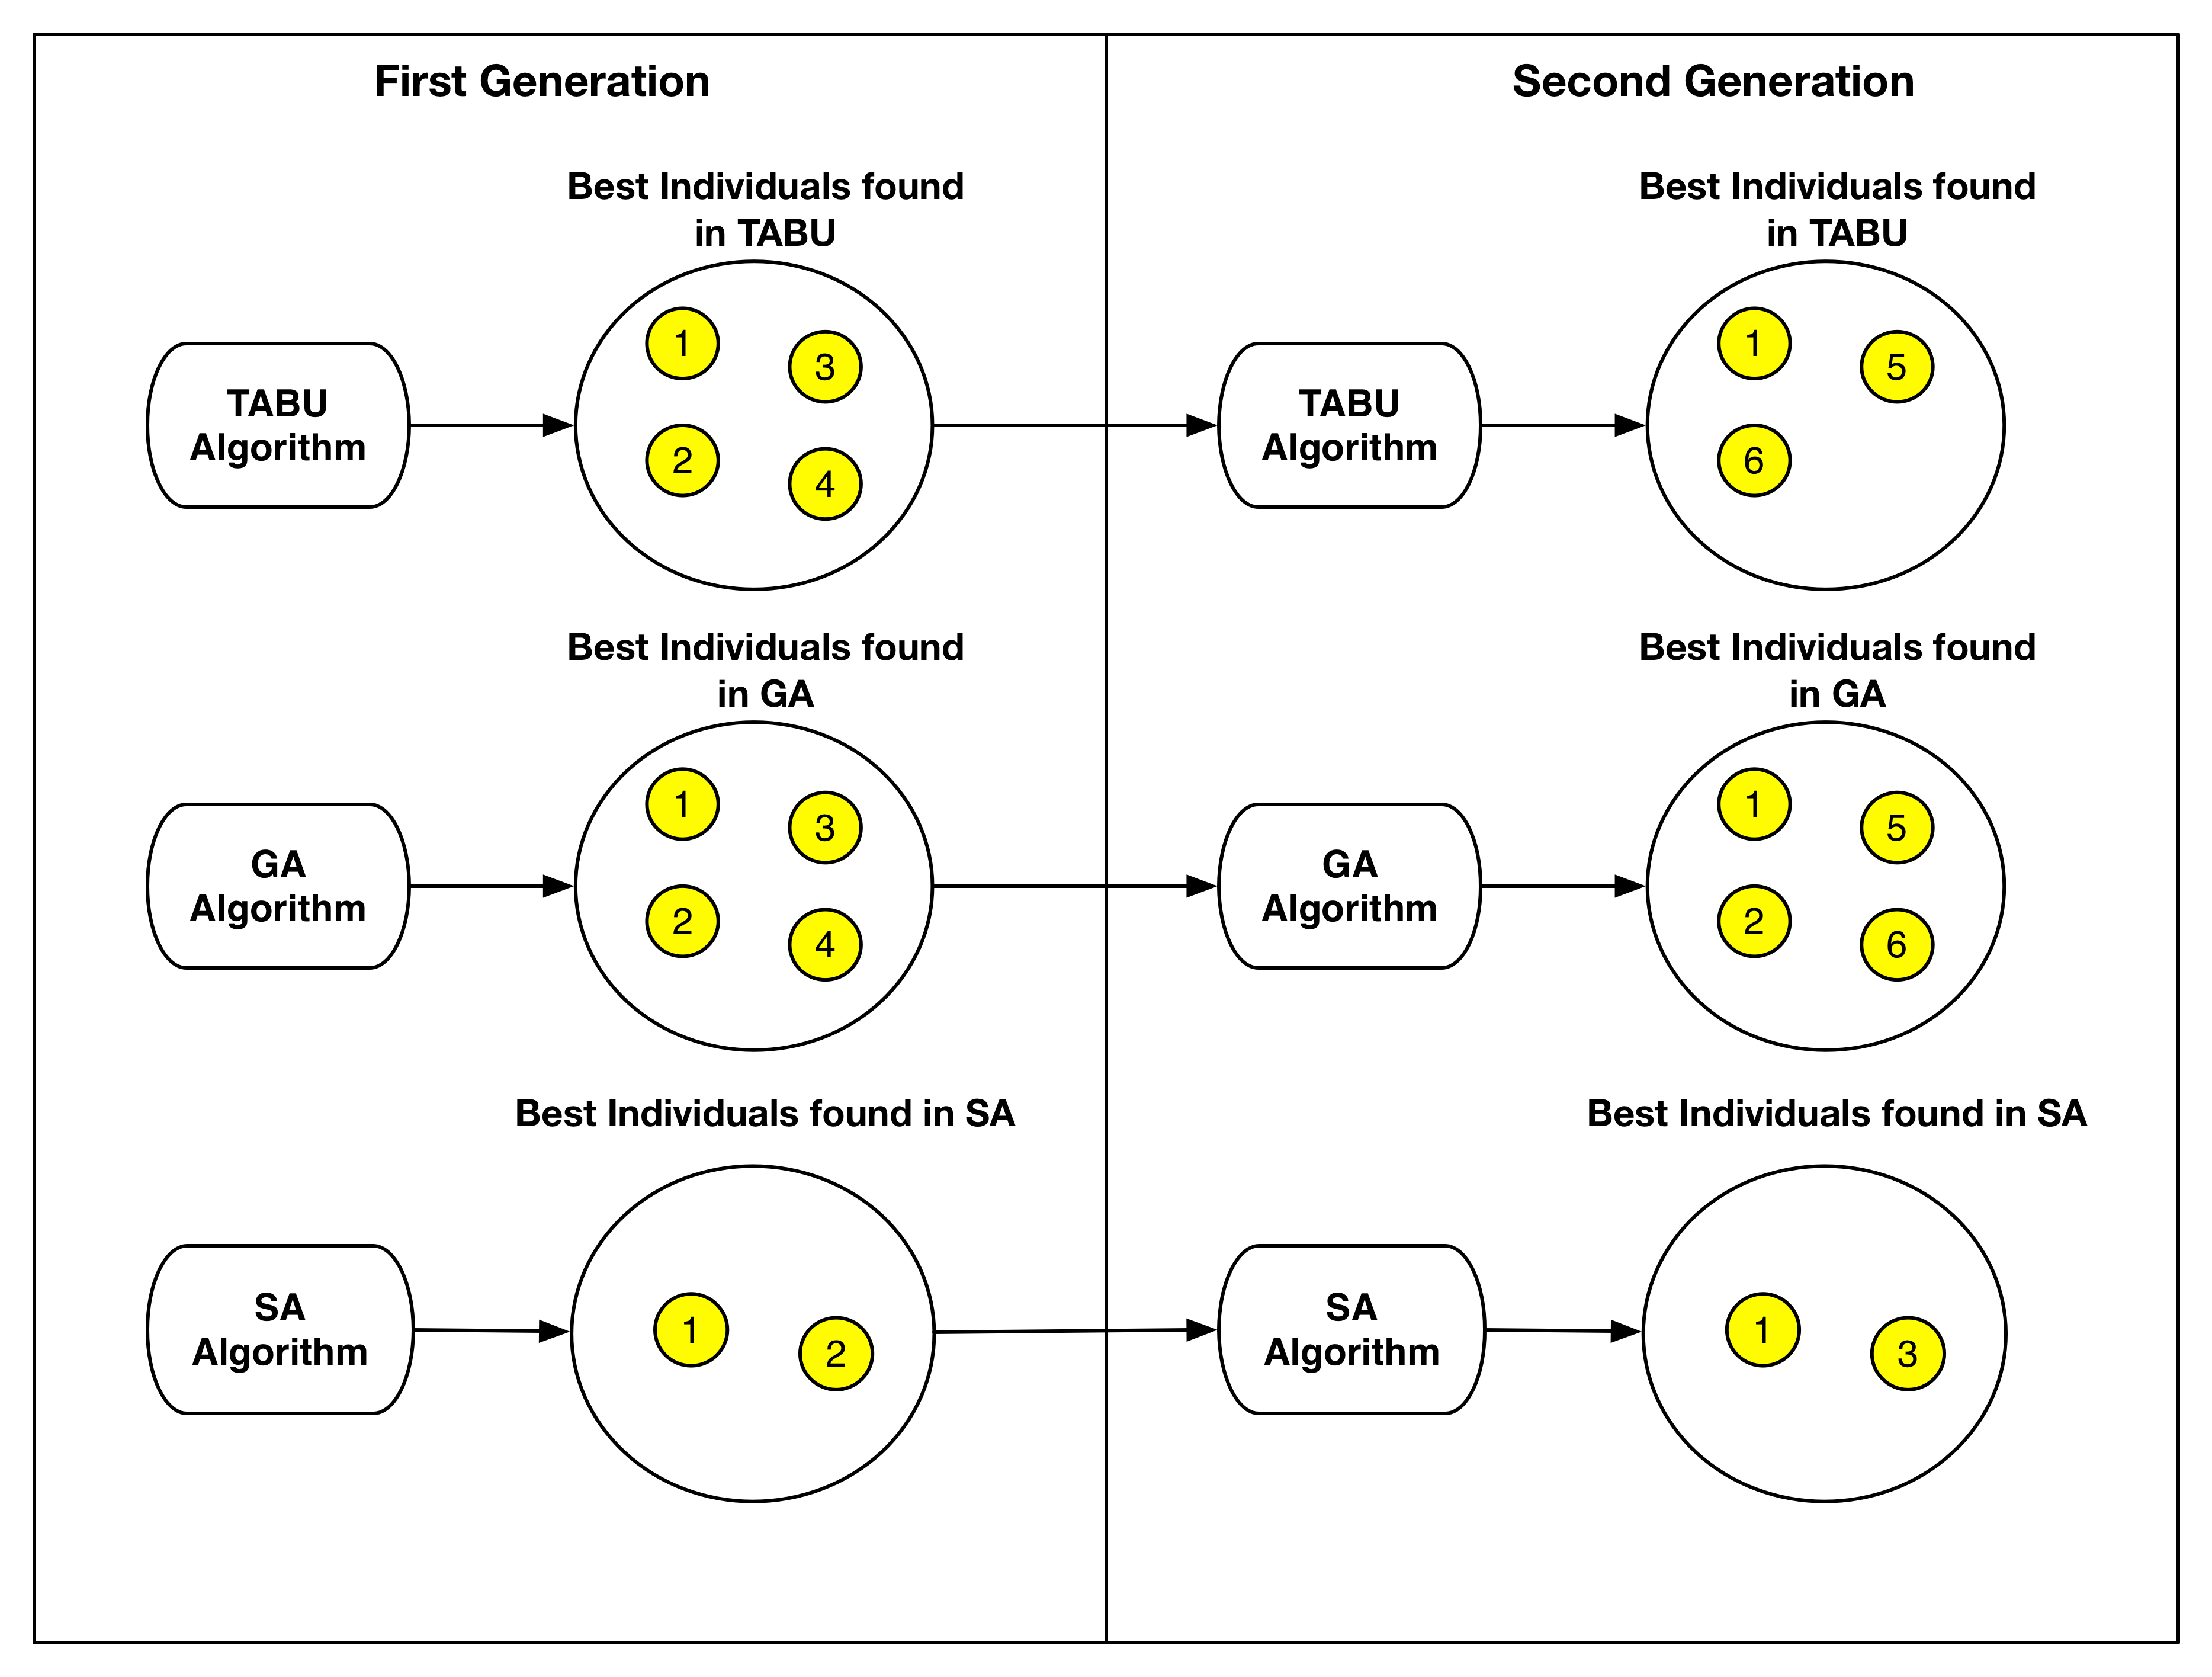
\includegraphics[width=0.8\linewidth]{independ.png}
\end{figure}
\end{frame}



\begin{frame}
\frametitle{IAdapter-Collaborative Approach}
\begin{figure}[H]
\centering
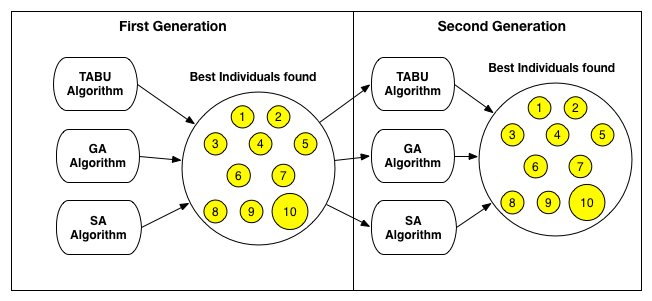
\includegraphics[width=1\linewidth]{collaborative.png}
\end{figure}
\end{frame}


\begin{frame}
\frametitle{IAdapter-Genotype Representation}
\begin{figure}[H]
\centering
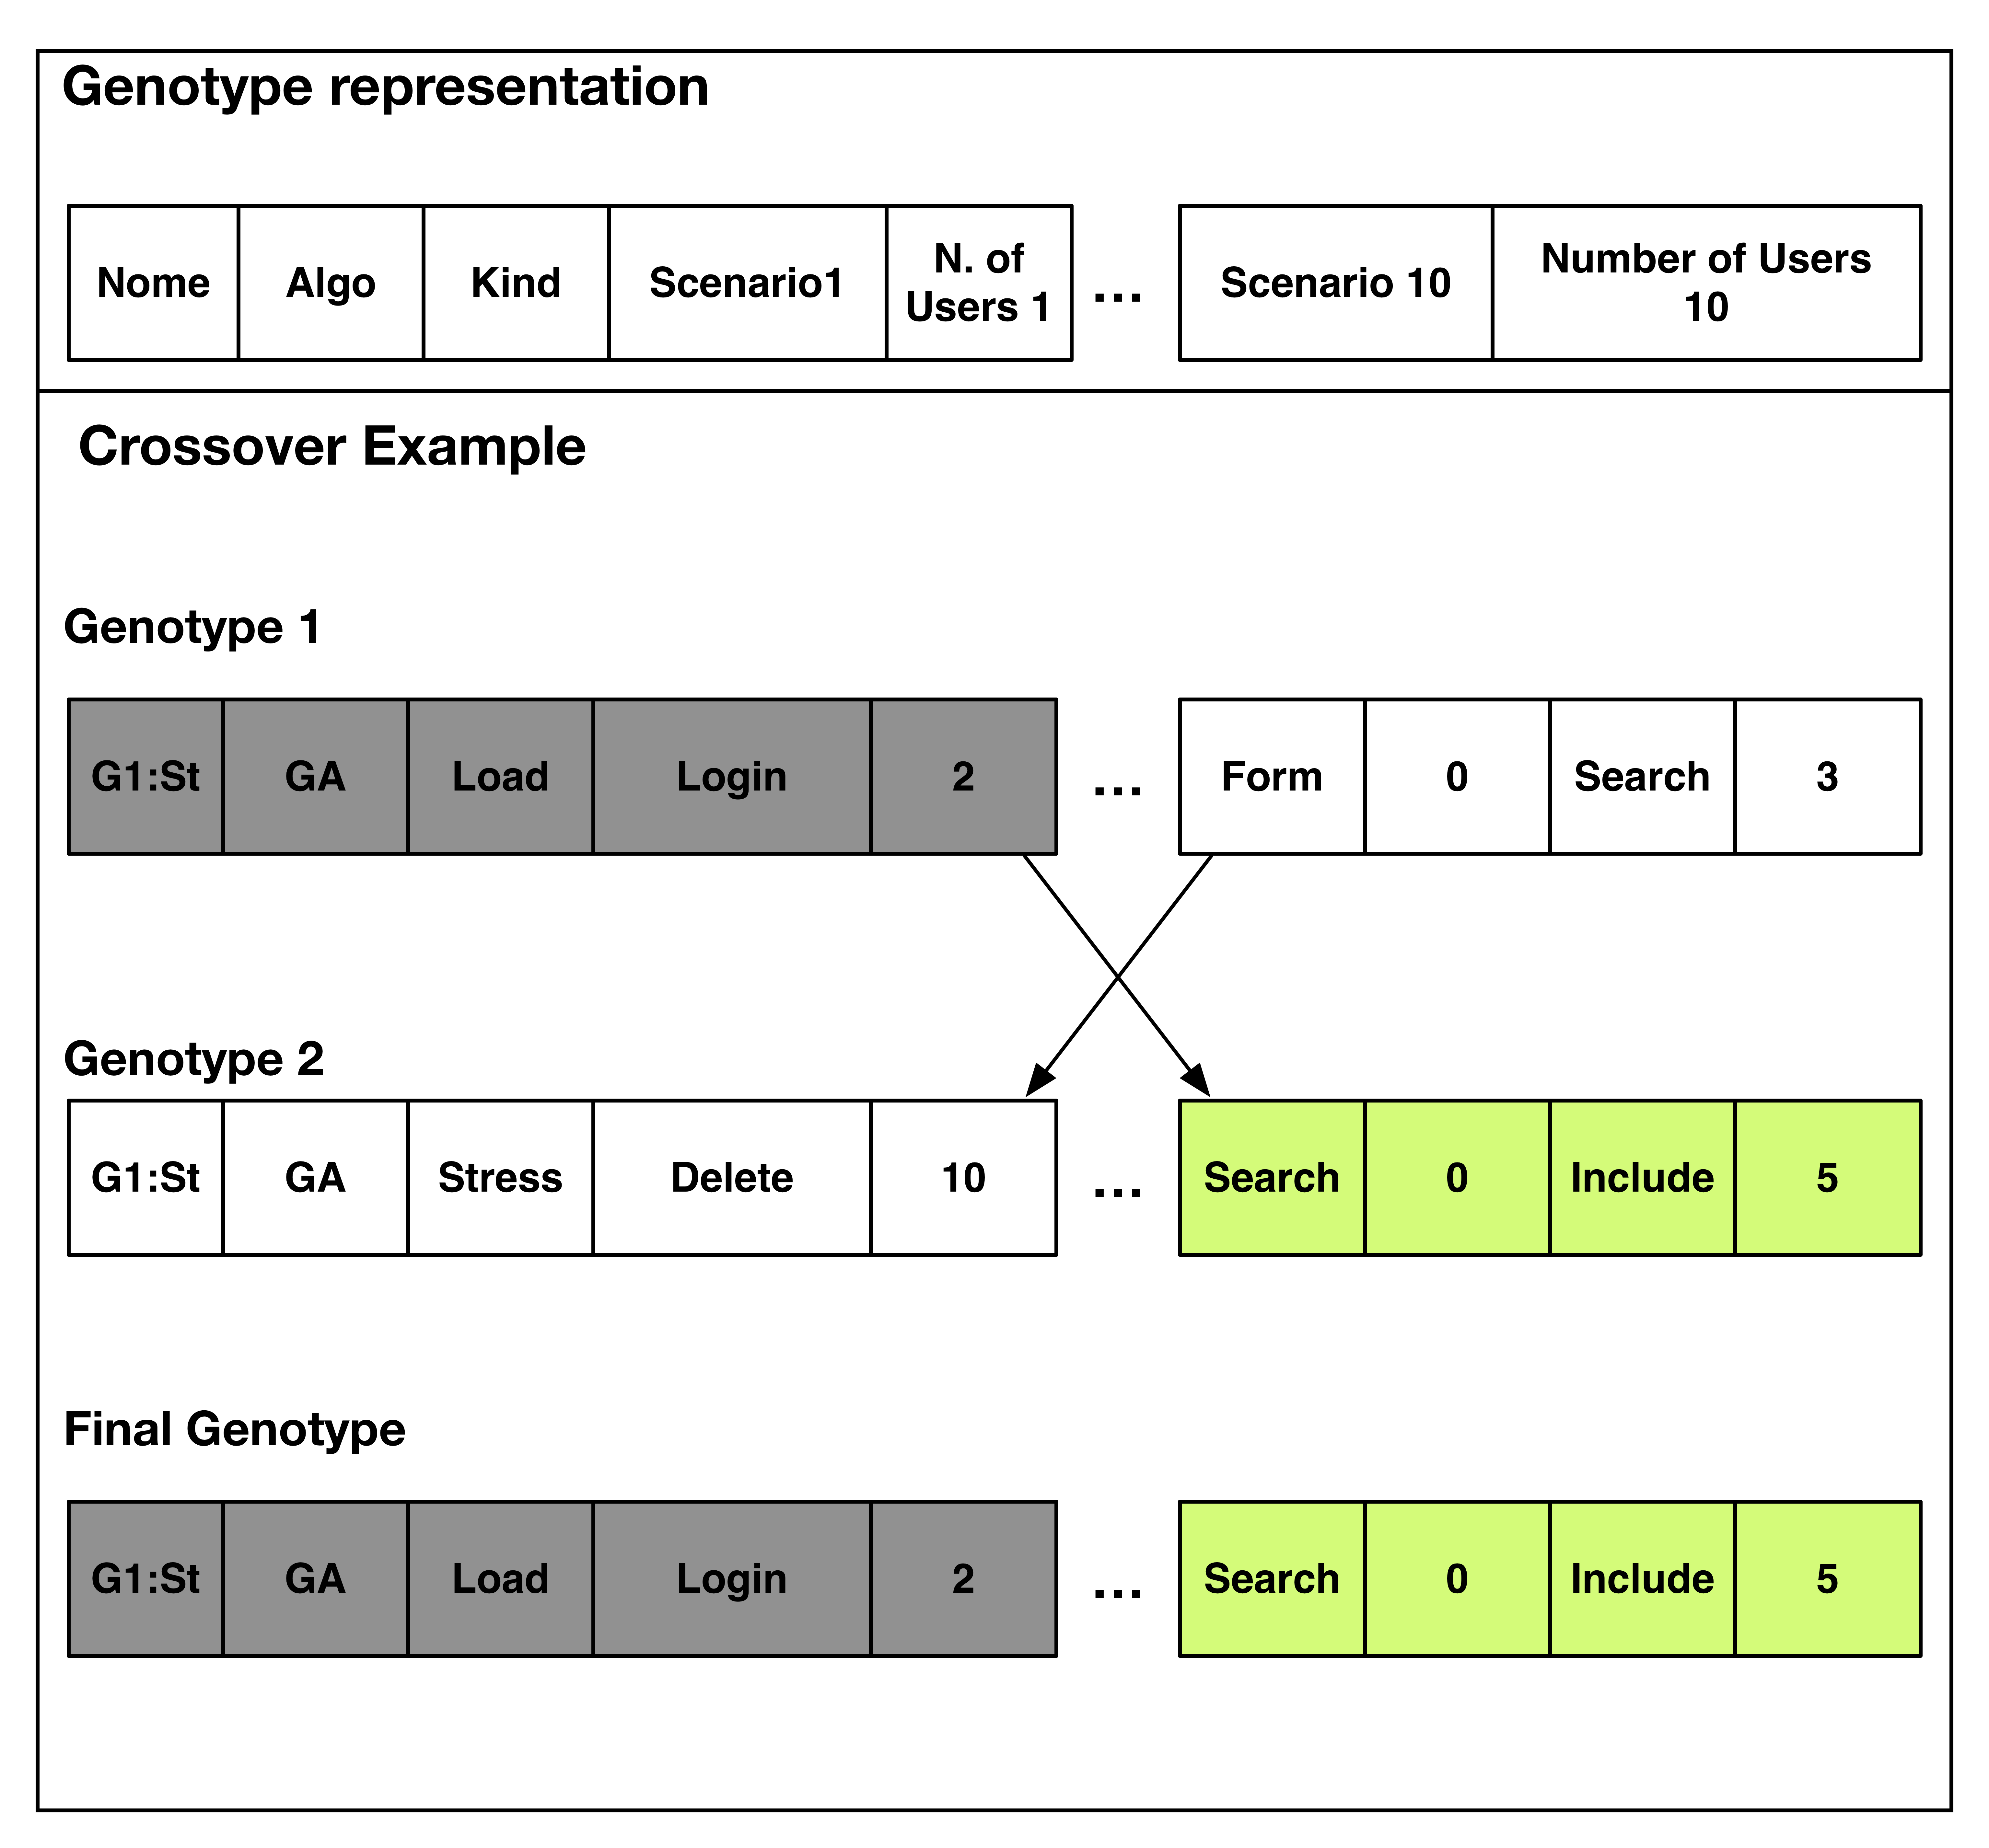
\includegraphics[width=0.7\linewidth]{genomerepresentation.png}
\end{figure}
\end{frame}

\begin{frame}
\frametitle{IAdapter-Tabu Search}
\begin{figure}[H]
\centering
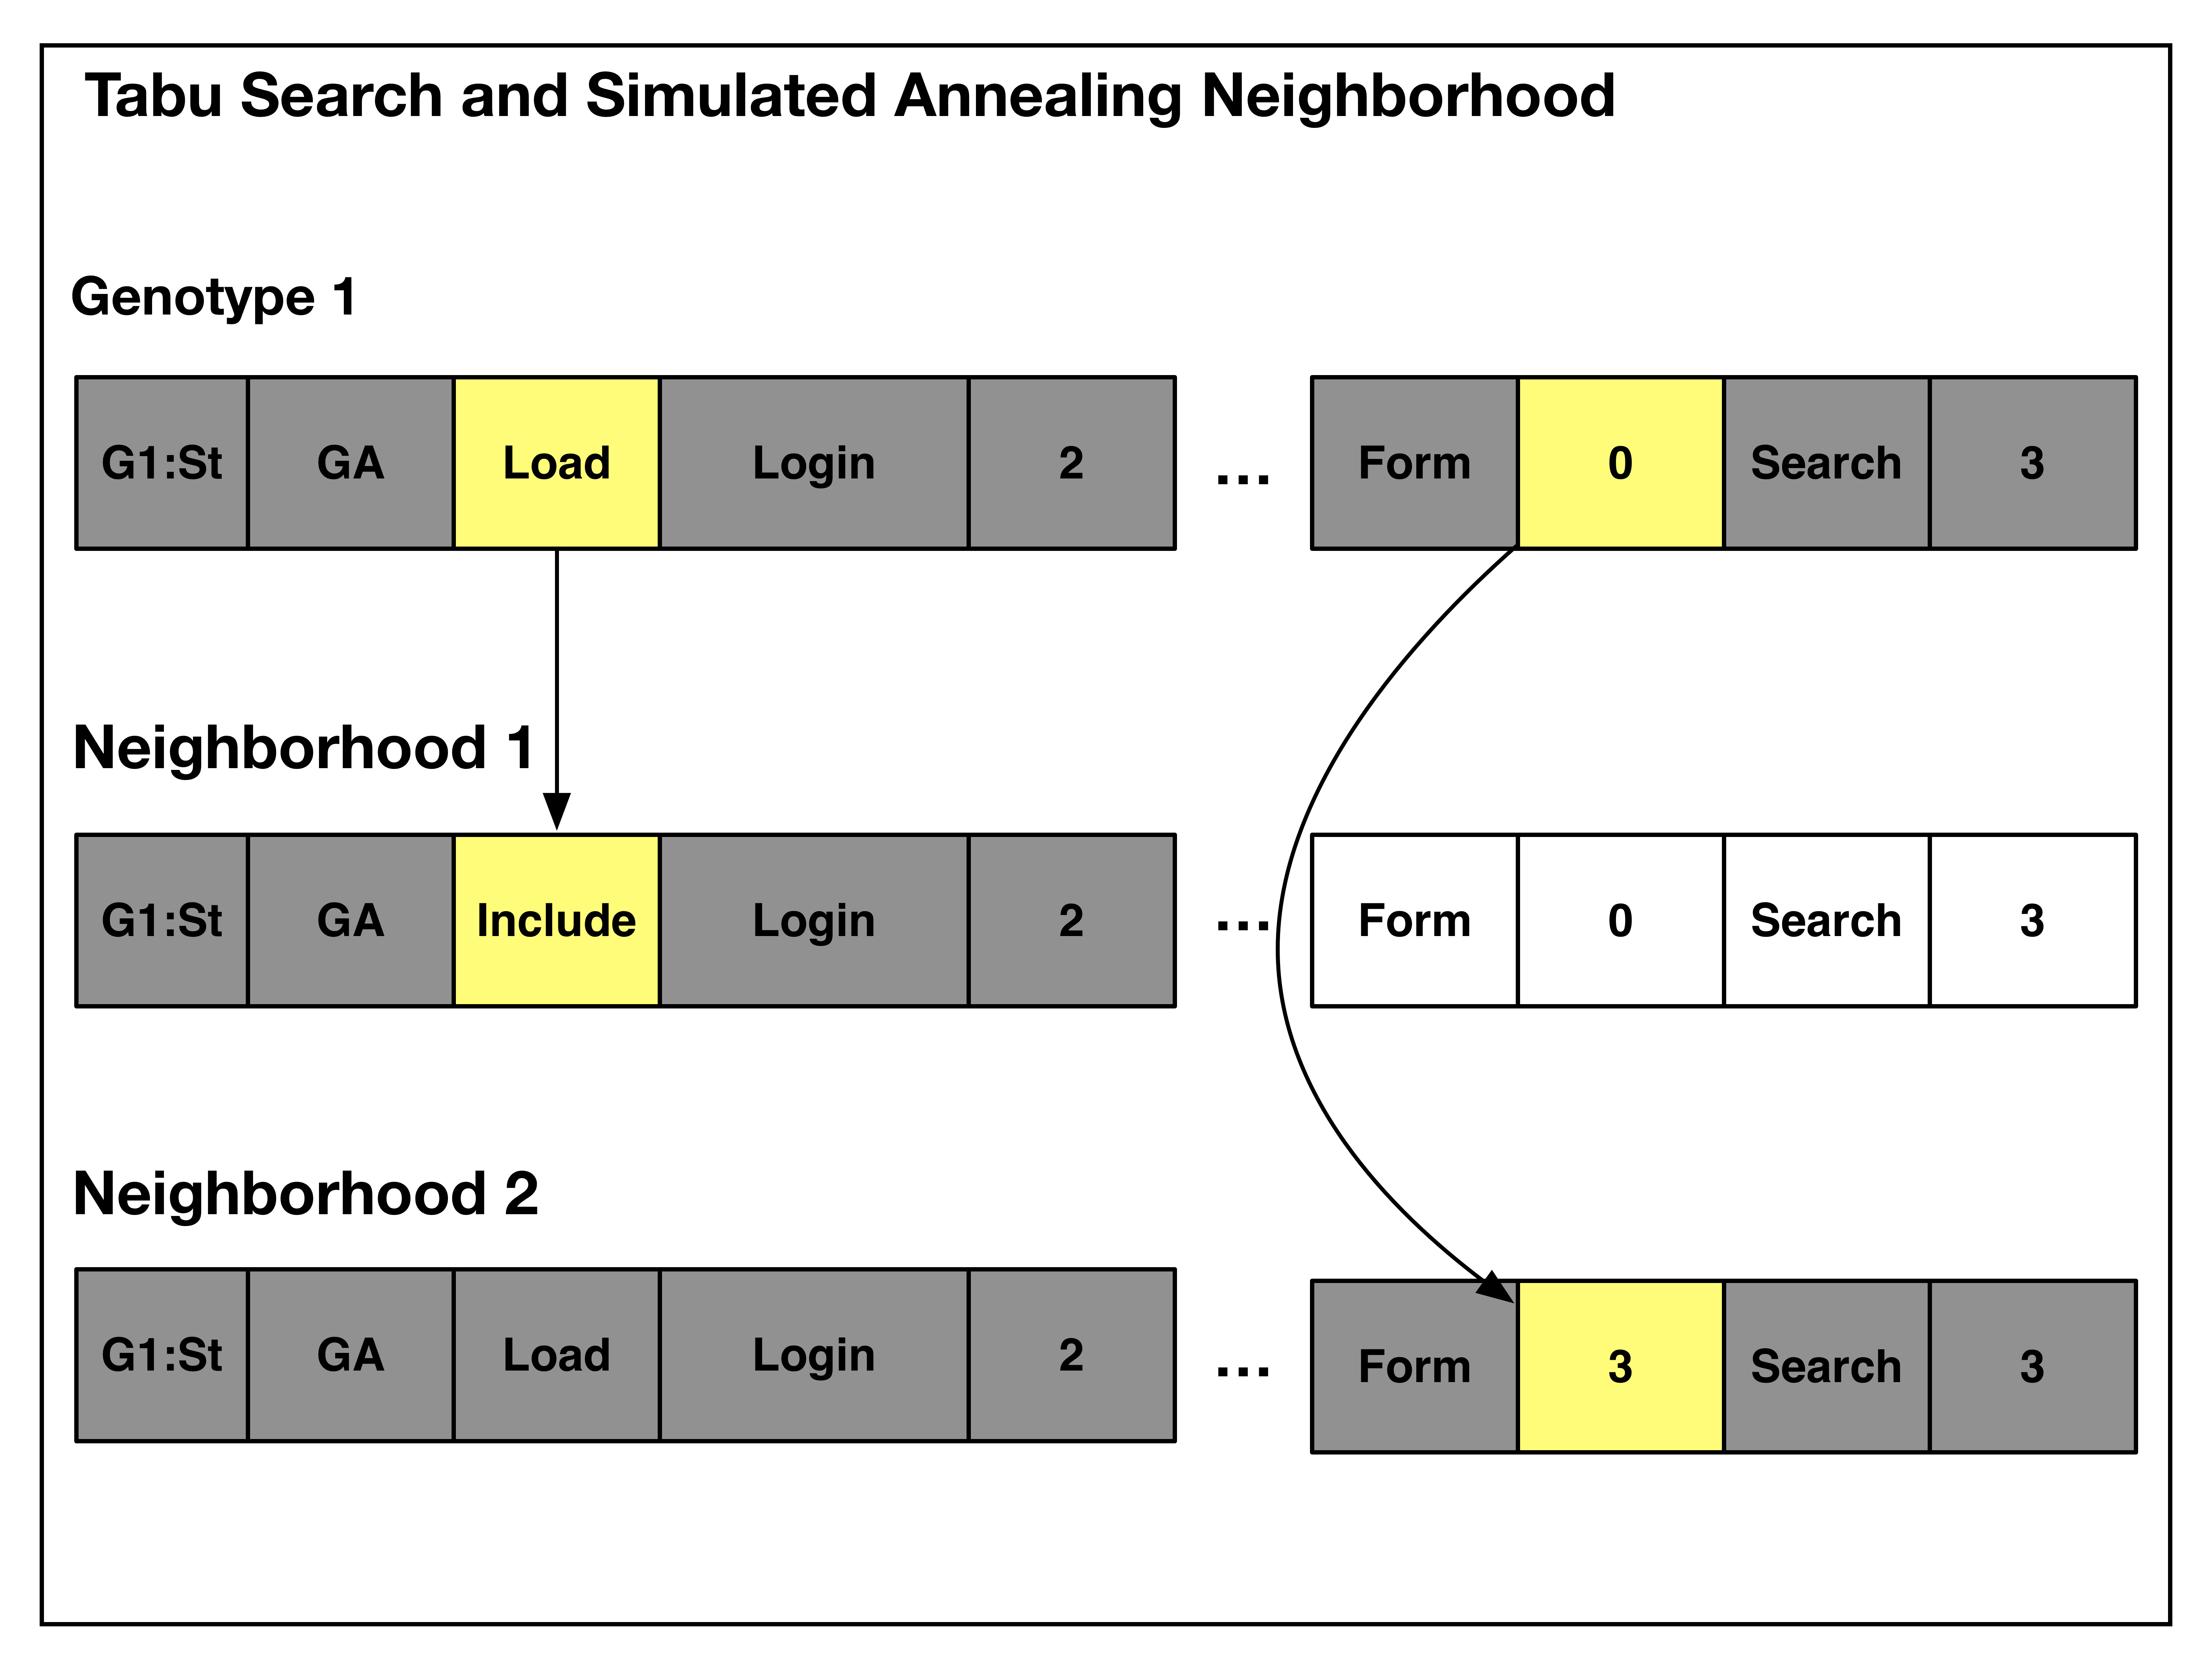
\includegraphics[width=0.7\linewidth]{TabuNE.png}
\end{figure}
\end{frame}

\begin{frame}
\frametitle{IAdapter-Fitness Function}
\begin{figure}[H]
\centering
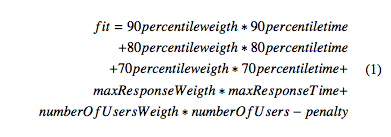
\includegraphics[width=1.1\linewidth]{fit1.png}
\end{figure}
\end{frame}


\section{Experiments}

\begin{frame}
\frametitle{Experiments}
\begin{itemize}
\item The first experiment has implemented 27 generations;
\item The second experiment has performed 6 generations;
\item 300 executions by generation (100 times for each algorithm), generating 300 new individuals;
\item The experiments had used a initial population of 100 individuals;
\item The Genetic Algorithm used the top 10 individuals from each generation to the crossover operation;
\item The Tabu List has been configured with the size of 10 individuals and expire every 2 generations;
\item The mutation operation was applied to 10\% of the population on each generation.
\end{itemize}
\end{frame}


\begin{frame}
\frametitle{First Experiment}
\begin{figure}[H]
\centering
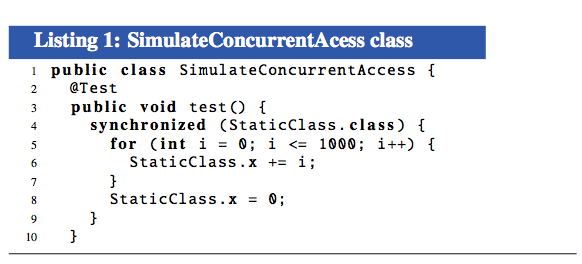
\includegraphics[width=0.8\linewidth]{classe.png}
\end{figure}
\end{frame}


\begin{frame}[allowframebreaks]
\frametitle{First Experiment}
\begin{table}[h]
\centering
\caption{Fitness function maximum value by algorithm (90\% percentile)}
\label{tab:averagefirst}
\begin{tabular}{|l|l|l|l|l|}
\hline
GEN & HM & TS  & GA    & SA    \\ \hline
1          & 11238 & 11238         & 11238 & 11238 \\ \hline
2          & 11804 & 11596         & 11801 & 10677 \\ \hline
3          & 11787 & 8932          & 8411  & 10869 \\ \hline
4          & 11723 & 9753          & 9611  & 10760 \\ \hline
5          & 8164  & 9780          & 10738 & 4794  \\ \hline
6          & 11802 & 9781          & 11086 & 6120  \\ \hline
\end{tabular}
\end{table}
\end{frame}


\begin{frame}[allowframebreaks]
\frametitle{First Experiment}
\begin{table}[h]
\centering
\caption{Fitness function maximum value by algorithm (90\% percentile)}
\label{tab:averagefirst}
\begin{tabular}{|l|l|l|l|l|}
\hline
GEN & HM & TS  & GA    & SA    \\ \hline
7          & 9985  & 5782          & 11272 & 11798 \\ \hline
8          & 11803 & 11749         & 10084 & 11309 \\ \hline
9          & 11806 & 7284          & 11633 & 10766 \\ \hline
10         & 11807 & 9386          & 11717 & 4557  \\ \hline
11         & 11802 & 9653          & 11802 & 11151 \\ \hline
12         & 11807 & 10594         & 11793 & 9434  \\ \hline
13         & 11802 & 10848         & 10382 & 11805 \\ \hline
14         & 11801 & 11551         & 7219  & 10237 \\ \hline
15         & 11807 & 1701          & 7189  & 9338  \\ \hline
16         & 11813 & 6203          & 11758 & 5321  \\ \hline
17         & 11805 & 10720         & 10805 & 11748 \\ \hline
\end{tabular}
\end{table}
\end{frame}

\begin{frame}[allowframebreaks]
\frametitle{First Experiment}
\begin{table}[h]
\centering
\caption{Fitness function maximum value by algorithm (90\% percentile)}
\label{tab:averagefirst}
\begin{tabular}{|l|l|l|l|l|}
\hline
GEN & HM & TS  & GA    & SA    \\ \hline
18         & 9600  & 6371          & 11698 & 7818  \\ \hline
19         & 11733 & 8160          & 11648 & 11509 \\ \hline
20         & 9589  & 9428          & 11805 & 4813  \\ \hline
21         & 11800 & 9463          & 11798 & 10801 \\ \hline
22         & 11805 & 11799         & 11804 & 6029  \\ \hline
23         & 11836 & 11655         & 11800 & 3579  \\ \hline
24         & 11805 & 11512         & 11803 & 5761  \\ \hline
25         & 11804 & 11573         & 11802 & 9680  \\ \hline
26         & 11800 & 11575         & 11403 & 9388  \\ \hline
27         & 11805 & 10691         & 11745 & 9465  \\ \hline
\end{tabular}
\end{table}
\end{frame}


\begin{frame}
\frametitle{Wilcoxon Test}

\begin{itemize}
\item The Wilcoxon signed-rank test is a non-parametric statistical hypothesis test used when comparing two related samples, matched samples, or repeated measurements on a single sample to assess whether their population mean ranks differ.

\item The Wilcoxon test applied in the first experiment showed a significant advantage of hybrid using metaheuristic approach.
\end{itemize}

\end{frame}

\begin{frame}
\frametitle{Second Experiment}
\begin{figure}[H]
\centering
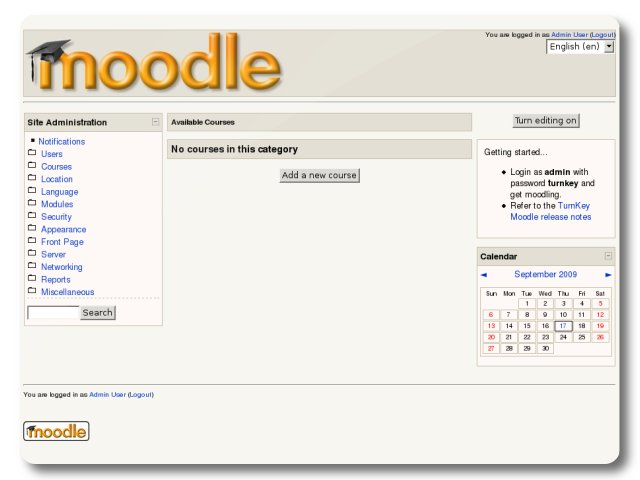
\includegraphics[width=0.8\linewidth]{moodle.jpg}
\end{figure}
\end{frame}


\begin{frame}
\frametitle{Moodle Scenarios}
\begin{itemize}
\item PostDeleteMessage- This scenario post and delete messages in the moodle application.
\item  MyHome- This scenario access the user’s homepage of the application.
\item Login- This scenario are responsible by the user authentica- tion of the application.
\item Notifications- This scenario enter in the notification page of each user.
\item Start Page- Initial start page of the application.
\item Badge- This scenario enter in the Badge page.
\end{itemize}
\end{frame}


\begin{frame}
\frametitle{Second Experiment}
\begin{figure}[H]
\centering
\includegraphics[width=1\linewidth]{generationcomparative.PNG}
\end{figure}
\end{frame}

\begin{frame}
\frametitle{Second Experiment}
\begin{figure}[H]
\centering
\includegraphics[width=0.8\linewidth]{gened.PNG}
\end{figure}
\end{frame}


\begin{frame}[allowframebreaks]
\frametitle{Second Experiment}
\begin{table}[h]
\centering
\caption{Results obtained from the second experiment}
\label{tab:secondexperiment}
\begin{tabular}{|l|l|l|l|l|}
\hline
GEN & HM    & TS    & GA    & SA    \\
\hline
1          & 32242 & 32242 & 32242 & 32242 \\
\hline
2          & 34599 & 32443 & 26290 & 35635 \\
\hline
3          & 35800 & 34896 & 34584 & 34248 \\
\hline
4          & 35782 & 34912 & 32689 & 25753 \\
\hline
5          & 35611 & 31833 & 34631 & 8366  \\
\hline
6          & 35362 & 35041 & 33397 & 9706 \\
\hline
\end{tabular}
\end{table}
\end{frame}

\begin{frame}
\frametitle{Second Experiment}
\begin{figure}[H]
\centering
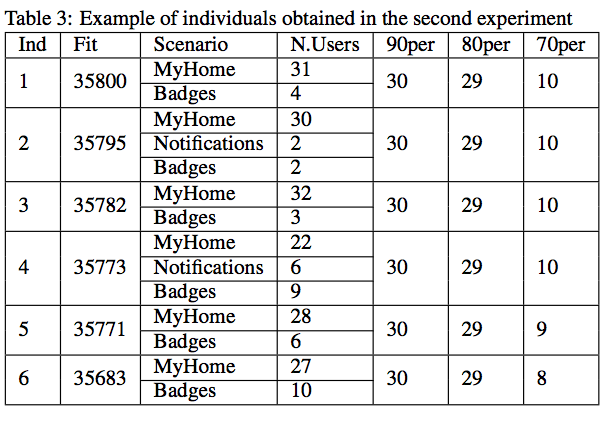
\includegraphics[width=0.8\linewidth]{ind1.PNG}
\end{figure}
\end{frame}

\section{Schedule}

\begin{frame}
\frametitle{Schedule}
\begin{figure}[H]
\centering
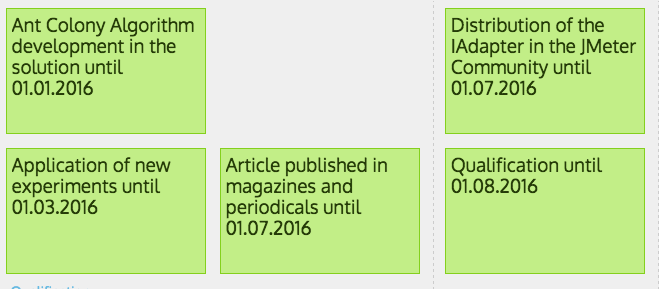
\includegraphics[width=1\linewidth]{stories3.PNG}
\end{figure}
\end{frame}

\begin{frame}
\frametitle{Schedule}
\begin{figure}[H]
\centering
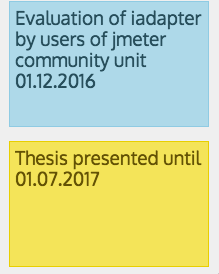
\includegraphics[width=0.5\linewidth]{stories2.PNG}
\end{figure}
\end{frame}




\section{Conclusion}

\begin{frame}
\frametitle{Conclusion}

\begin{itemize}
\item This research presented a approach of use Hybrid Metaheuristc in load, performance and stress testing
\item Two experiments were performed to validate the solution. The first experiment has been applied in an emulated component and the second experiment has been applied in an installed Moodle application.
\item The collaborative approach has obtained better fit values in both experiments.
\end{itemize}
\end{frame}


\section{References}

\begin{frame}[allowframebreaks]
\frametitle{Bibliografia}
\bibliographystyle{apalike}
\bibliography{biblioteca}

\end{frame}


\end{document}
